\section{Сравнение моделей освещения}

Модели освещения делятся на \emph{глобальные} и \emph{локальные}~\cite{CGPaP}.

Глобальные модели учитывают не только свет, исходящий непосредственно из источника, но и освещение, отражающееся от других объектов на сцене, что позволяет получать более реалистичные изображения.

Локальные модели, в свою очередь, учитывают только свет исходящий из источника. На цвет выходного пикселя влияет лишь интенсивность света и свойства поверхности.

Для целей данной работы достаточно использовать локальную модель освещения. Рассмотрим несколько из них.

\subsection{Модель Фонга}

Модель Фонга --- это локальная~\cite{CGPaP} модель освещения, которая учитывает как диффузную составляющую модели освещения, так и зеркальную. Это позволяет достичь большего реализма, отобразив блики, появляющиеся на моделях под определённым углом наблюдения.

Модель Фонга основывается на модели Ламберта, которая позволяла определить лишь диффузное освещение. На такой модели поверхность имела одинаковую интенсивность на всей своей площади.

Математические принципы данной модели можно понять, если использовать рисунок~\ref{fig:fong}.

\begin{figure}[h]
    \centering
    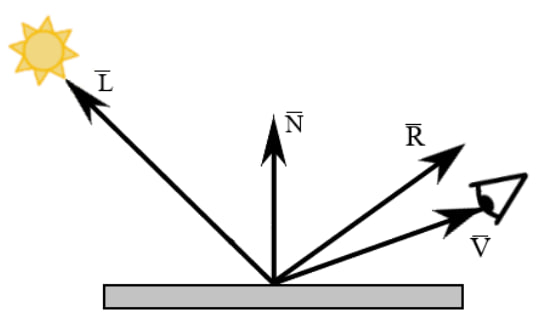
\includegraphics[width=.5\textwidth]{fong.jpg}
    \caption{Модель освещения Фонга}
    \label{fig:fong}
\end{figure}

На этом рисунке:
\begin{itemize}
    \item $\vec{L}$ --- вектор от точки на поверхности до источника света;
    \item $\vec{N}$ --- вектор нормали к поверхности в данной точке; 
    \item $\vec{R}$ --- вектор отражённого света;
    \item $\vec{V}$ --- вектор от точки на поверхности до наблюдателя (камеры);
\end{itemize}

Тогда интенсивность пикселя, отображающего данную точку на экране будет вычисляться согласно уравнению~\ref{eq:intens}.

\begin{equation}
    I = I_p \cdot K_a + I_0 \cdot K_b \cdot cos(\vec{L}, \vec{N}) + I_0 \cdot K_c \cdot cos^\alpha(\vec{R}, \vec{V})  
    \label{eq:intens}
\end{equation}

где $I$~---~итоговая интенсивность пикселя, отображающего данную точку на экране, $I_p$~---~интенсивность рассеянного света, $I_0$~---~интенсивность источника света, $K_a, K_b, K_c$~---~коэффициенты рассеянного, диффузного и зеркального освещения соответственно, $\alpha$~---~коэффициент блеска. 

$K_a, K_b, K_c, \alpha$ являются параметрами поверхности и, соответственно, константами. 

$I_p, K_a$ --- параметры модели освещения и тоже являются константами.

\subsection{Модель с картами освещения}

Модель с картами освещения --- это метод ускорить вычисления интенсивности освещения путём вычисления большинства параметров в момент построения сцены~\cite{LightMaps}. Такая модель может работать только в сценах, где положение объектов и источника(ов) освещения статичны. Сам метод сильно похож на метод теневых карт, однако вместо сохранения освещённости области изображения, будут сохранены значения векторов падающих на поверхность (и отражённых) лучей. 

Этот метод можно использовать вместе с моделью Фонга, чтобы значительно ускорить визуализацию очередного кадра.

Карту освещения, как и карту теней, придётся рассчитывать заново только если переместится источник света. В этот момент можно будет рассчитать все слагаемые из формулы~\ref{eq:intens} кроме последнего, а в последнем слагаемом останется рассчитать лишь косинус угла между векторами.

\subsection{Вывод}

В этой работе я буду использовать модель освещения Фонга с ускорением, использующим метод карт освещения. Поскольку построение реалистичного изображения не является целью работы, использовать более сложные (глобальные) модели освещения не нужно.